\documentclass{article}

\usepackage{geometry}
\usepackage{hyperref}
\usepackage{graphicx}
\usepackage{float}
\usepackage{cite}
\usepackage{graphicx}
\title {CS 201: Data Structures II \\Merkle Tree} % Mention your project title

\author{L2 Group 2} % Mention your team name
\date{Spring 2023}  

\begin{document}
\maketitle
\section{Group Members}
% Mention your Group Members and their ids
\begin{enumerate}
  \item Ayila Emad
  \item Daniyal
  \item Dua Batool
  \item Rohan Raj
\end{enumerate}
\section{Data Structure}
We will be using Merkle tree which is a tree-like hash-based data structure where each leaf node represents a hash value of a piece of data. Every other node represents the hash value of the concatenation of its child nodes in a recursive hashing process, with the root node representing as single hash value that is considered as the summary of the dataset. The Merkle Tree is commonly used to verify the integrity and authenticity of large datasets. 
\section{Application}
\begin{enumerate}
    \item \textbf{File systems:} Merkle trees can be used in file systems to efficiently verify the integrity of large files. Instead of having to hash the entire file, a Merkle tree can be constructed, allowing for efficient verification of the integrity of the file.
    \item \textbf{Blockchain technology:} Merkle trees are widely used in blockchain technology to ensure the authenticity and integrity of transactions and blocks in the blockchain. Each block in the blockchain contains a Merkle tree of the transactions in that block, and the root hash of this tree is included in the block header.
    \item \textbf{Version control systems:} Merkle trees are used in version control systems, such as Git, to efficiently track changes to large code repositories. In Git, each commit contains a Merkle tree of the changes made to the codebase, allowing for efficient verification of the integrity of the codebase.
\end{enumerate}
\section{Functionality}
\begin{enumerate}
    \item \textbf{Insertion} This function allows the user to insert a new data element into the Merkle Tree. Once inserted, the Merkle tree is updated by recalculating the hash values for the nodes along the path from the inserted leaf node to the root node of the tree.
    \item \textbf{Deletion} This function allows the user to delete a data element from the Merkle Tree. Once deleted, the Merkle tree is updated by recalculating the hash values for the nodes along the path from the inserted leaf node to the root node of the tree.
    \item \textbf{Verification} This function allows the user to verify the integrity of a data element or a set of data elements in the Merkle Tree. The user can verify whether a particular data element is present in the Merkle Tree and whether the data element has been tampered with using the hash values.
    \item \textbf{Hashing} This function allows the user to compute the hash of a data element or a set of data elements in the Merkle Tree. The hash value is used to verify the integrity of the data element or to compare it with other data elements in the Merkle Tree.
    \item \textbf{Merkle Proof} This function allows the user to generate a Merkle Proof, which is a set of hash values that can be used to prove the inclusion or non-inclusion of a data element in the Merkle Tree. The Merkle Proof can be used to provide evidence that a particular data element is present or absent in the Merkle Tree without revealing the actual data element.
\end{enumerate}

\begin{figure}[h]
    \centering
    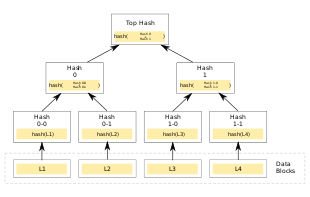
\includegraphics[scale = 1]{Hash_Tree.png}
\end{figure}

\newpage
\section{Datasets}
    \begin{enumerate}
     \item \textbf{For file storage and sharing:}\\ •	The Large Movie Review Dataset: This dataset contains a set of movie reviews that can be used to implement a Merkle Tree for storing and verifying the integrity of the reviews. The dataset is available for download from the following link: \\$https://ai.stanford.edu/~amaas/data/sentiment/$  \\
        •	The Reuters News Dataset: This dataset contains a large collection of news articles that can be used to implement a Merkle Tree for storing and verifying the integrity of the articles. The dataset is available for download from the following link: \\$https://archive.ics.uci.edu/ml/datasets/reuters-21578+text+categorization+collection$ 
        
        \item \textbf{For blockchain technology:} \\ •	Bitcoin Blockchain Dataset: This dataset contains a full historical record of all Bitcoin transactions, which can be used to demonstrate the usage of a Merkle Tree in validating the integrity of transactions in a blockchain network. Link: \\$https://www.kaggle.com/bigquery/bitcoin-blockchain$
        \\•	Ethereum Blockchain Dataset: This dataset contains a full historical record of all Ethereum transactions, which can be used to demonstrate the usage of a Merkle Tree in validating the integrity of smart contracts and transactions in a blockchain network. Link: \\$https://www.kaggle.com/bigquery/ethereum-blockchain$ 
        
\end{enumerate}

\newpage
\section{Work Distribution}
\begin{center}
  \begin{table}[h]
    \centering
    \begin{tabular}{|c|c|c|}
      \hline
      Item & Activity   & ID      \\ \hline
      1    & Working & ae07352 \\ \hline
      2    & Working & db07098 \\ \hline
      3    & Functionality & d07605 \\ \hline
      4    & Functionality & rr07656 \\ \hline
    \end{tabular}

    \label{tab:my-table6}
  \end{table}
\end{center}
\section{Attribution}
OpenAI. (2021). ChatGPT [Computer software]
\newline
Simplilearn. (n.d.). Merkle Tree in Blockchain. Simplilearn. 
\newline
Pandey, S. (2018, August 9). Merkle Tree: A Simple Explanation and Implementation. 
\newline
Davis, B. (2018, July 11). Applications of the Merkle Tree Data Structure. Medium. 
% \begin{thebibliography}{9}
%   \bibitem{chatgpt}
%   OpenAI. (2021). ChatGPT [Computer software]
%   \end{thebibliography}
\end{document}
